\section{Auswertung}
\label{sec:Auswertung}

\subsection{Bestimmung des Schubmoduls G}

Zur Berechnung des Schubmoduls wird () verwendet.
Die Größen $m_k$ und $R_k$ waren mit Fehler am Gerät abzulesen,
die restlichen Größen ergeben sich als Mittelwert der gemessenen Werte:

\begin{table}
\centering
\caption{Gemessener Durchmesser des Drahtes}
\label{tab:Dicke}
\begin{tabular}{ c S[table-format=1.3] }
\toprule
$\text{Messung#}$ & $2R/mm$ \\
\midrule
1 & 0,185   \\
2 & 0,190   \\
3 & 0,185   \\
4 & 0,188   \\
5 & 0,191   \\
\midrule
Mittelwert () & 0,188 \\
Fehler () & 0,001\\
\bottomrule
\end{tabular}
\end{table}

\begin{table}
\centering
\caption{Gemessene Länge des Drahtes}
\label{tab:Dicke}
\begin{tabular}{ c S[table-format=2.1] }
\toprule
$\text{Messung#}$ & $L/cm$ \\
\midrule
1 & 60,0   \\
2 & 60.0   \\
3 & 60.1   \\
\midrule
Mittelwert () & 60.0 \\
Fehler () & 0.1 \\
\bottomrule
\end{tabular}
\end{table}

\begin{table}
\centering
\caption{Periodendauern ohne Magnetfeld}
\label{tab:Dauern}
\begin{tabular}{ c S[table-format=2.3] }
\toprule
$\text{Messung#}$ & $T/s$ \\
\midrule
1 & 18,065  \\
2 & 18,069  \\
3 & 18,055  \\
4 & 18,069  \\
5 & 18,053  \\
6 & 18,054  \\
7 & 18,063  \\
8 & 18,050  \\
9 & 18,057  \\
10 & 18,058 \\
\midrule
Mittelwert& 18,059 \\
Fehler () & 0,006\\
\bottomrule
\end{tabular}
\end{table}

Mit diesen Werten ergibt sich der Schubmodul als $G = num{7,278(4,24\%)e10}\si{\newton\per\meter\sqared}$
mit einem prozentualen Fehler von. Zusammen mit dem zuvor angegebenen Elastizitätsmodul
ergibt sich dann mit () die Querkontraktionszahlt als $\mu = 0,4427$
mit dem selben realtiven Fehler da E als fehlerfrei angenommer wird und es sich um einen linearen Zusammenhang handelt.

\subsection{Messung des Erdmagnetfelds}

Das Magnetfeld von Helmholtz-Spulen ergibt sich ähnlich zu langen Spule durch ()
mit den angegebenen Werten $N = \num{390}$ und $R_H = \num{78}\si{\mili\meter}$.
Die Periodendauern aus Tabelle(\ref{tab:DauernB}) werden werden im folgenden gegen $\frac{1}{T^2}$ aufgetragen:
\begin{figure}
  \centering
  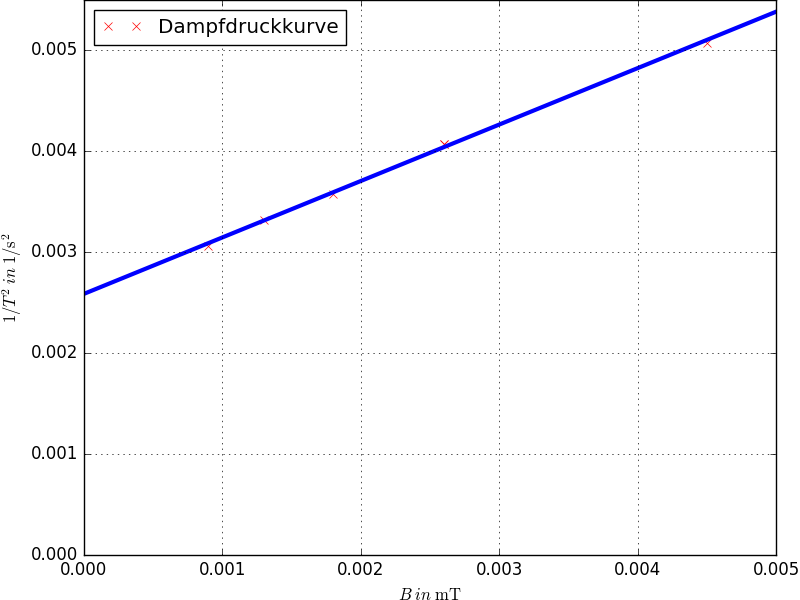
\includegraphics[width=\textwidth]{figure102.pdf}
  \caption{$\frac{1}{T^2}$ aufgetragen gegen die das Magntfeld $B$.}
  \label{fig:1}
\end{figure}
Die mit linearer Regression ausgerechnete Steigung der Geraden ist hier nach ()
\begin{equation*}
  T = 2\pi\sqrt{\frac{\Theta}{mB+D}}
  \frac{1}{T^2} =k(mB+D) \text{mit} k=\frac{1}{4\pi^2\Theta}
\text{und es folg für das magnetische Moment}
 m_mgn = km = \num{2,96(0,06)e-3}   \si{\Ampere\meter\squared}
\end{equation*}
Und aus dem Achsen-Abschnitt ergibt sich $D = num{2,587(0,028)e-3}\si{\per\second\squareds}$

\begin{table}
\centering
\caption{Periodendauern mit Helmholz-Spulen}
\label{tab:DauernB}
\begin{tabular}{ c S[table-format=1.1] S[table-format=1.1] S[table-format=2.3] }
\toprule
$\text{Messung#}$ & $I/A$ & $B/mT$ & $T/s$ \\
\midrule
1 &   &     & 14,044  \\
2 &   &     & 14,054  \\
3 & 1 & 4,5 & 14,034  \\
4 &   &     & 14,015  \\
5 &   &     & 14,017  \\
\midrule
Mittelwert ()  & & & 14,033 \\
Fehler ()      & & & 0,017        \\
\midrule
1 &     &       & 15,688  \\
2 &     &       & 15,673  \\
3 & 0,6 & 2,6   & 15,655  \\
4 &     &       & 15,675  \\
5 &     &       & 15,652  \\
\midrule
Mittelwert ()  & & & 15,668 \\
Fehler ()      & & &   0,015      \\
\midrule
1 &      &      & 16,738  \\
2 &      &      & 16,732  \\
3 & 0,4  & 1,8  & 16,722  \\
4 &      &      & 16,746  \\
5 &      &      & 16,714  \\
\midrule
Mittelwert ()  & & & 16,730 \\
Fehler ()       & & &    0,013                   \\
\midrule
1 &     &     & 17,354  \\
2 &     &     & 17,345  \\
3 & 0,3 & 1,3 & 17,331  \\
4 &     &     & 17,359  \\
5 &     &     & 17,344  \\
\midrule
Mittelwert ()  & & & 17,347 \\
Fehler ()      & & &   0,011                     \\
\midrule
1 &     &     & 18,092  \\
2 &     &     & 18,092  \\
3 & 0,2 & 0,9 & 18,064  \\
4 &     &     & 18,047  \\
5 &     &     & 18,041  \\
\midrule
Mittelwert () & & & 18,067\\
Fehler ()     & & &  0,024     \\
\bottomrule
\end{tabular}
\end{table}

Mit Hilfe des berechneten $m$ kann nun das Erdmagnetfeld mit den gemessenen Werten bestimmt werden (\ref{tab:DauernE}).
Zuvor wird aber das gesamte Trägheitsmoment des Systems benötigt um () nach B umstellen zu können.
\begin{align*}
\Theta_{\text{ges}} = \Theta_{\text{Kugel}} + \Theta_k &= \frac{2}{5}m_k R_k^2 + \Theta_k =
 \num{1,34e-4}\si{\kilo\gramm\meter\squared}\\ 
\text{Damit ist B dann:}\\
B^* &=
 (\frac{1}{2\pi\DeltaT}+\sqrt{\frac{D}{\Theta})^2-\frac{D}{\Theta}} =  \num{4,58(0,09)e-3}\si{\tesla}
\end{align*}


\begin{table}
\centering
\caption{Periodendauern mit Erdmagnetfeld}
\label{tab:DauernE}
\begin{tabular}{ c S[table-format=2.3] }
\toprule
$\text{Messung#}$ & $T/s$ \\
\midrule
1 & 19,687  \\
2 & 19,686  \\
3 & 19,691  \\
4 & 19,699  \\
5 & 19,700  \\
6 & 19,700  \\
7 & 19,712  \\
8 & 19,712  \\
9 & 19,713  \\
10 & 19,720 \\
\midrule
Mittelwert ()  & 19,702\\
Fehler ()     &  0,012\\
\bottomrule
\end{tabular}
\end{table}

\section{Diskussion}
\label{sec:Diskussion}

Zwar besitzen die Zeitmessungen einehoh Präzision, doch nichsdesto trotz liegen die beiden gemessenen Werte für 
$D$ wie auch das errechnete Erdmagnetfeld (lit. $B^* = \num{30}\si{\mikro\tesla}$) um mehrere Größenordnungen außeinander, was entweder auf einen sehr massiven systematichen Fehler schließen lässt oder,
was wahrscheinlicher ist seinen Ursprung in der linearen Ausgleichsrecchnung hat; entweder durch eine erhebliche Verzerrung durch auftragen der Quadrate, 
unzuläsiges ansetzten der Kleinwinkelnäherung für $sin(\phi)$, oder einen tiefsitzenden Rechenfehler.
\end{document}
